

\section{Apnea}

\begin{frame}
\frametitle{Cos'\`e una apnea?}

\begin{itemize}
  \item
    \textcolor{blue}{Respirazione}
  \item
    \textcolor{blue}{Fasi respiratorie}: inspirazione, espirazione e pausa respiratoria.
  \item
    \textcolor{blue}{Apnea}: pausa respiratoria di durata uguale o maggiore di $10s$.
\end{itemize}

% \begin{definition}
% Una \alert{apnea} \`e una 
% \end{definition}
\end{frame}

\begin{frame}
  \frametitle{Sindrome da apnea del sonno}
\subsection{Sindrome da apnea del sonno}
\begin{center}
\begin{tikzpicture}
%   [scale=.8,auto=left,every node/.style={fill=blue!20}]
[->,>=stealth',shorten >=1pt,auto,node distance=3cm,
  thick,main node/.style={circle,fill=blue!20,draw,font=\sffamily\Large\bfseries}]


  \node (patologia) at 			(0,2) 	{patologia};

  \node (epidemiologia) at 		(3.7,0.5)		{epidemiologia};
  \node (diagnosi) at 			(4,2) 		{prassi diagnostica};
   \node (sintomatologia) at 		(3.8,3) 		{sintomatologia};


  \node (polisonnografia) at 		(8,2) 	{polisonnografia};
  \node (diffusione) at 		(8,0) 		{diffusione};
  \node (consapevolezza) at 		(8,1) 		{consapevolezza};


   \foreach \from/\to in {patologia/sintomatologia,patologia/epidemiologia,patologia/diagnosi,diagnosi/polisonnografia, epidemiologia/diffusione, epidemiologia/consapevolezza}
     \draw (\from) -- (\to);

\end{tikzpicture}
\end{center}
\end{frame}



\section{Motivazione}
  \subsection{Diagnosi e terapia d'emergenza}


  \begin{frame}
  \frametitle{Motivazione}
\endcenter

% \begin{description}
%   \item[Diagnosi]: Utile di per s\'e. Meno invasiva. Meno costosa.
%   \item[Terapia d'emergenza]:
%     Svegliare il soggetto. Come scegliere la soglia di allarme? Conviene svegliare il soggetto?
% \end{description}
% \begin{flushleft}
\begin{itemize}
 \item[] 
    \textcolor{blue}{Diagnosi}

    Utile di per s\'e. Meno invasiva. Meno costosa.
 \item[]
  \textcolor{blue}{Terapia d'emergenza}

  Svegliare il soggetto. Come scegliere la soglia di allarme? Conviene svegliare il soggetto?
\end{itemize}
% \end{flushleft}



% \begin{tikzpicture}
% %   [scale=.8,auto=left,every node/.style={fill=blue!20}]
% [->,>=stealth',shorten >=1pt,auto,node distance=3cm,
%   thick,main node/.style={circle,fill=blue!20,draw,font=\sffamily\Large\bfseries}]
% 
%   \node (diagnosi) at 		(0,2) 	{diagnosi};
%   \node (terapia) at 		(0,4) 	{terapia d'emergenza};
%   \node (utile) at 		(4,1.5) {utile di per se};
%   \node (menoInvasiva) at 	(4,2) 	{meno invasiva};
%   \node (economica) at 		(4,2.5) {pi\`u economica};% di una polisonnografia classica
%   \node (svegliare) at 		(4,4) 	{svegliare il soggetto};
%   
% 
%    \foreach \from/\to in {diagnosi/utile,terapia/svegliare,diagnosi/menoInvasiva,diagnosi/economica}
%      \draw (\from) -- (\to);
% 
% \end{tikzpicture}
\end{frame}


    
% La sindrome da apnea del sonno \`e una patologia molto diffusa. 
% Il sonno di un soggetto affetto da tale patologia \`e disturbato da apnee e da episodi di respirazione insufficiente. 
% Forme medie e gravi di sindrome da apnea del sonno sono un fattore di rischio per, e una concausa di: pressione alta, malattie cardiache, diabete, depressione. 
% Inoltre tale patologia contribuisce a creare una senso perenne di sonnolenza e spossatezza. 
% Si stima che pi\`u della met\`a dei soggetti affetti da tale patologia non ne siano al corrente\cite{intrrr}. 
% Questo a causa dei meccanismi di diagnosi pi\`u diffusi che sono costosi o scomodi e richiedono al paziente di trascorrere la notte in un centro specializzato.
% Inoltre i centri specializzati sono pochi e possono essere molto costosi. 
% Sono in fase di sviluppo ma non hanno per il momento una diffusione capillare altri strumenti di diagnosi pi\`u pratici. 
% Alcuni studi hanno analizzato i dati di alcuni soggetti che sono morti a causa di eventi cardiovascolari acuti e che erano 
% affetti da forme medie o gravi di sindrome da apnea del sonno. 
% La conclusione \`e stata che la maggior parte di tali soggetti \`e morta durante il sonno. 
% In questa tesi sviluppiamo un prototipo di uno strumento non invasivo di monitoraggio del respiro e di diagnosi della sindrome da apnea del sonno: attraverso uno stetoscopio elettronico, il sistema deve vigilare su un soggetto e registrare la frequenza e la durata delle apnee e, cosa pi\`u importante, deve svegliare il soggetto nel caso in cui l'apnea duri troppo. 


\subsection{Svegliare il soggetto}
\begin{frame}
    \frametitle{Conviene svegliare il soggetto?}
    \framesubtitle{Motivi empirici\footnote{\emph{Day–Night Pattern of Sudden Death in Obstructive Sleep Apnea.} 
  	Apoor S. Gami, Daniel E. Howard, Eric J. Olson, and Virend K. Somers.
  	The new england journal of medicine.} e biologici}
\begin{center}
\begin{figure}
 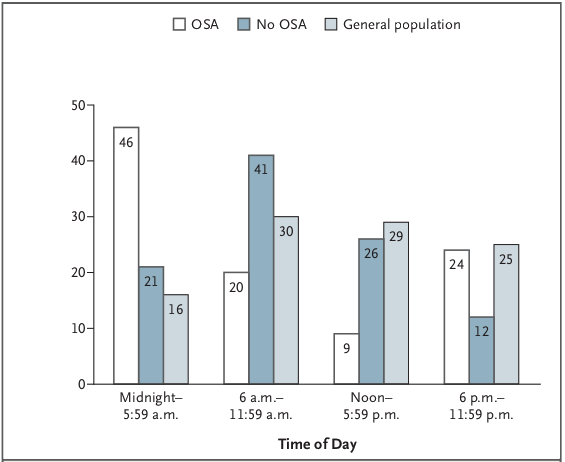
\includegraphics[height=0.65\textheight]{./daynight2.png}
 % daynight.xcf: 566x589 pixel, 72dpi, 19.97x20.78 cm, bb=0 0 566 589
\end{figure}
\end{center}
% non dice che i soggetti hanno una apnea immediatamente prima di morire, per questo c'e' bisogni di ulteriori esperimenti fatti da una equipe medica

\end{frame}

% \begin{frame}
%     \frametitle{Conviene svegliare il soggetto?}
%     \framesubtitle{Motivi biologici}
% 
% % \begin{itemize}
% % \item 2 is prime (two divisors: 1 and 2).
% % \pause
% % \item 3 is prime (two divisors: 1 and 3).
% % \pause
% % \item 4 is not prime (\alert{three} divisors: 1, 2, and 4).
% % \end{itemize}
% 
% \end{frame}
% 



% \subsection{Scelta della soglia}
% \begin{frame}
%   \frametitle{Scelta della soglia}
% \begin{tikzpicture}
% [->,>=stealth',shorten >=1pt,auto,node distance=3cm, thick,main node/.style={circle,fill=blue!20,draw,font=\sffamily\Large\bfseries}]
% \node (soglia) at (0,1.5) {soglia di allarme};
% \node (apnea) at (3.7,3) {definizione di apnea};
% \node (ipossiemia) at (4,1) {ipossiemia};
% \node (tradeoff) at (3.8,2) {trade off};
% \node (variabile) at (3.4, 0) {variabile};
% 
%    \foreach \from/\to in {soglia/tradeoff,soglia/apnea,soglia/ipossiemia, soglia/variabile}
%       \draw (\from) -- (\to);
% \end{tikzpicture}
% \end{frame}

